


\chapter{DIMENSIONAMIENTO DEL CABLE DE CARGA}
\section{Selección de material.} % section headings are printed smaller than chapter names

\makebox[\textwidth]{Hilo – Latón Cu63 Zn37} \par

Se escogió este material ya que es un material bastante sencillo de caracterizar y por supuesto se observa claramente la deformación. Buscamos muchos tipos de hilos, como es de algodón, acero inoxidable etc. , pero el que más se encajaba en cuanto a nuestras características fue este material 
Para la caracterización del material de manera experimental se utilizó el peso que tenemos de base y se fue agregando litro por litro hasta llegar a los 5.300 kg. 

\begin{center}
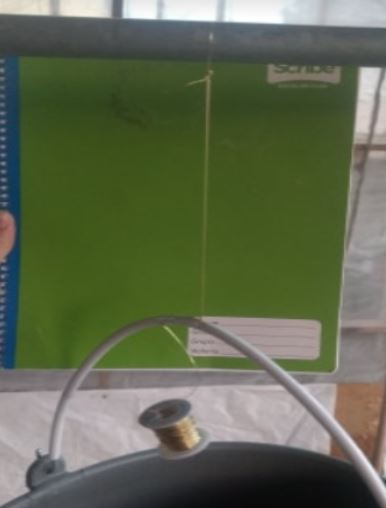
\includegraphics[width=.3\linewidth]{C/figs/A_1.jpg}
\quad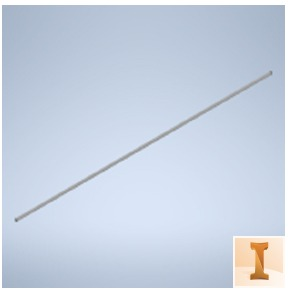
\includegraphics[width=.3\linewidth]{C/figs/A_2.jpg}
\\[\baselineskip]% adds vertical line spacing
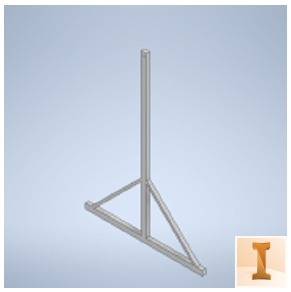
\includegraphics[width=.3\linewidth]{C/figs/A_3.jpg}
\quad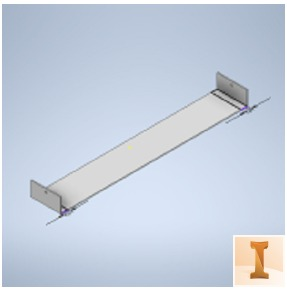
\includegraphics[width=.3\linewidth]{C/figs/A_4.jpg}
\end{center}

\textrm{Se tomó de base para la caracterización 10 cm exactos, ya agregandole los 5.3 kg se obtuvo un desplazamiento de 1 mm en el cable.}


\section{Esfuerzo y deformación máxima.}

\begin{table}[htb]
\centering
\begin{tabular}{| p{2.8cm}| p{2.8cm} |}
\hline
\multicolumn{2}{|c|}{Latón Cu63 Zn37} \\
\hline
E &  $\sigma$y \\
\hline \hline
100-115 GPa & 300-700 MPa  \\ \hline
\end{tabular}
\caption{Propiedades mecánicas}
\label{}
\end{table}

\begin{center}
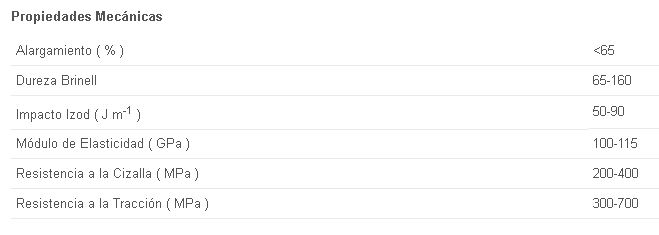
\includegraphics[width=1\linewidth]{C/figs/B_1.jpg} 
\end{center}


\section{Deformación total considerando flexión de \\viga y deformación axial del cable con carga de diseño.}
\begin{center}
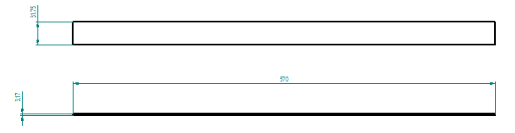
\includegraphics[width=.8\linewidth]{C/figs/B_2.jpg} 
\end{center}

